\section{Auswertung}
\label{sec:Auswertung}

\subsection{Lange Spule}

Im folgenden wird die magnetische Flussdichte einer langen Spule gemessen und graphisch dargestellt.
%\begin{minipage}{0.5\textwidth}
\begin{table}
\centering
\caption{Messdaten der langen Spule}
\begin{tabular}{c c}
  \toprule
  x (m) &  B (10e-3 T) \\
  \midrule
  -0.02 &         0.23 \\
  -0.01 &         0.28 \\
  -0.01 &         0.35 \\
  -0.01 &         0.46 \\
    0.00 &         0.60 \\
    0.01 &         0.84 \\
    0.01 &         1.15 \\
    0.01 &         1.43 \\
    0.02 &         1.70 \\
    0.03 &         1.89 \\
    0.03 &         2.02 \\
    0.04 &         2.12 \\
    0.04 &         2.18 \\
  \bottomrule
\end{tabular}
\end{table}
%\end{minipage}

%\begin{minipage}{0.5\textwidth}
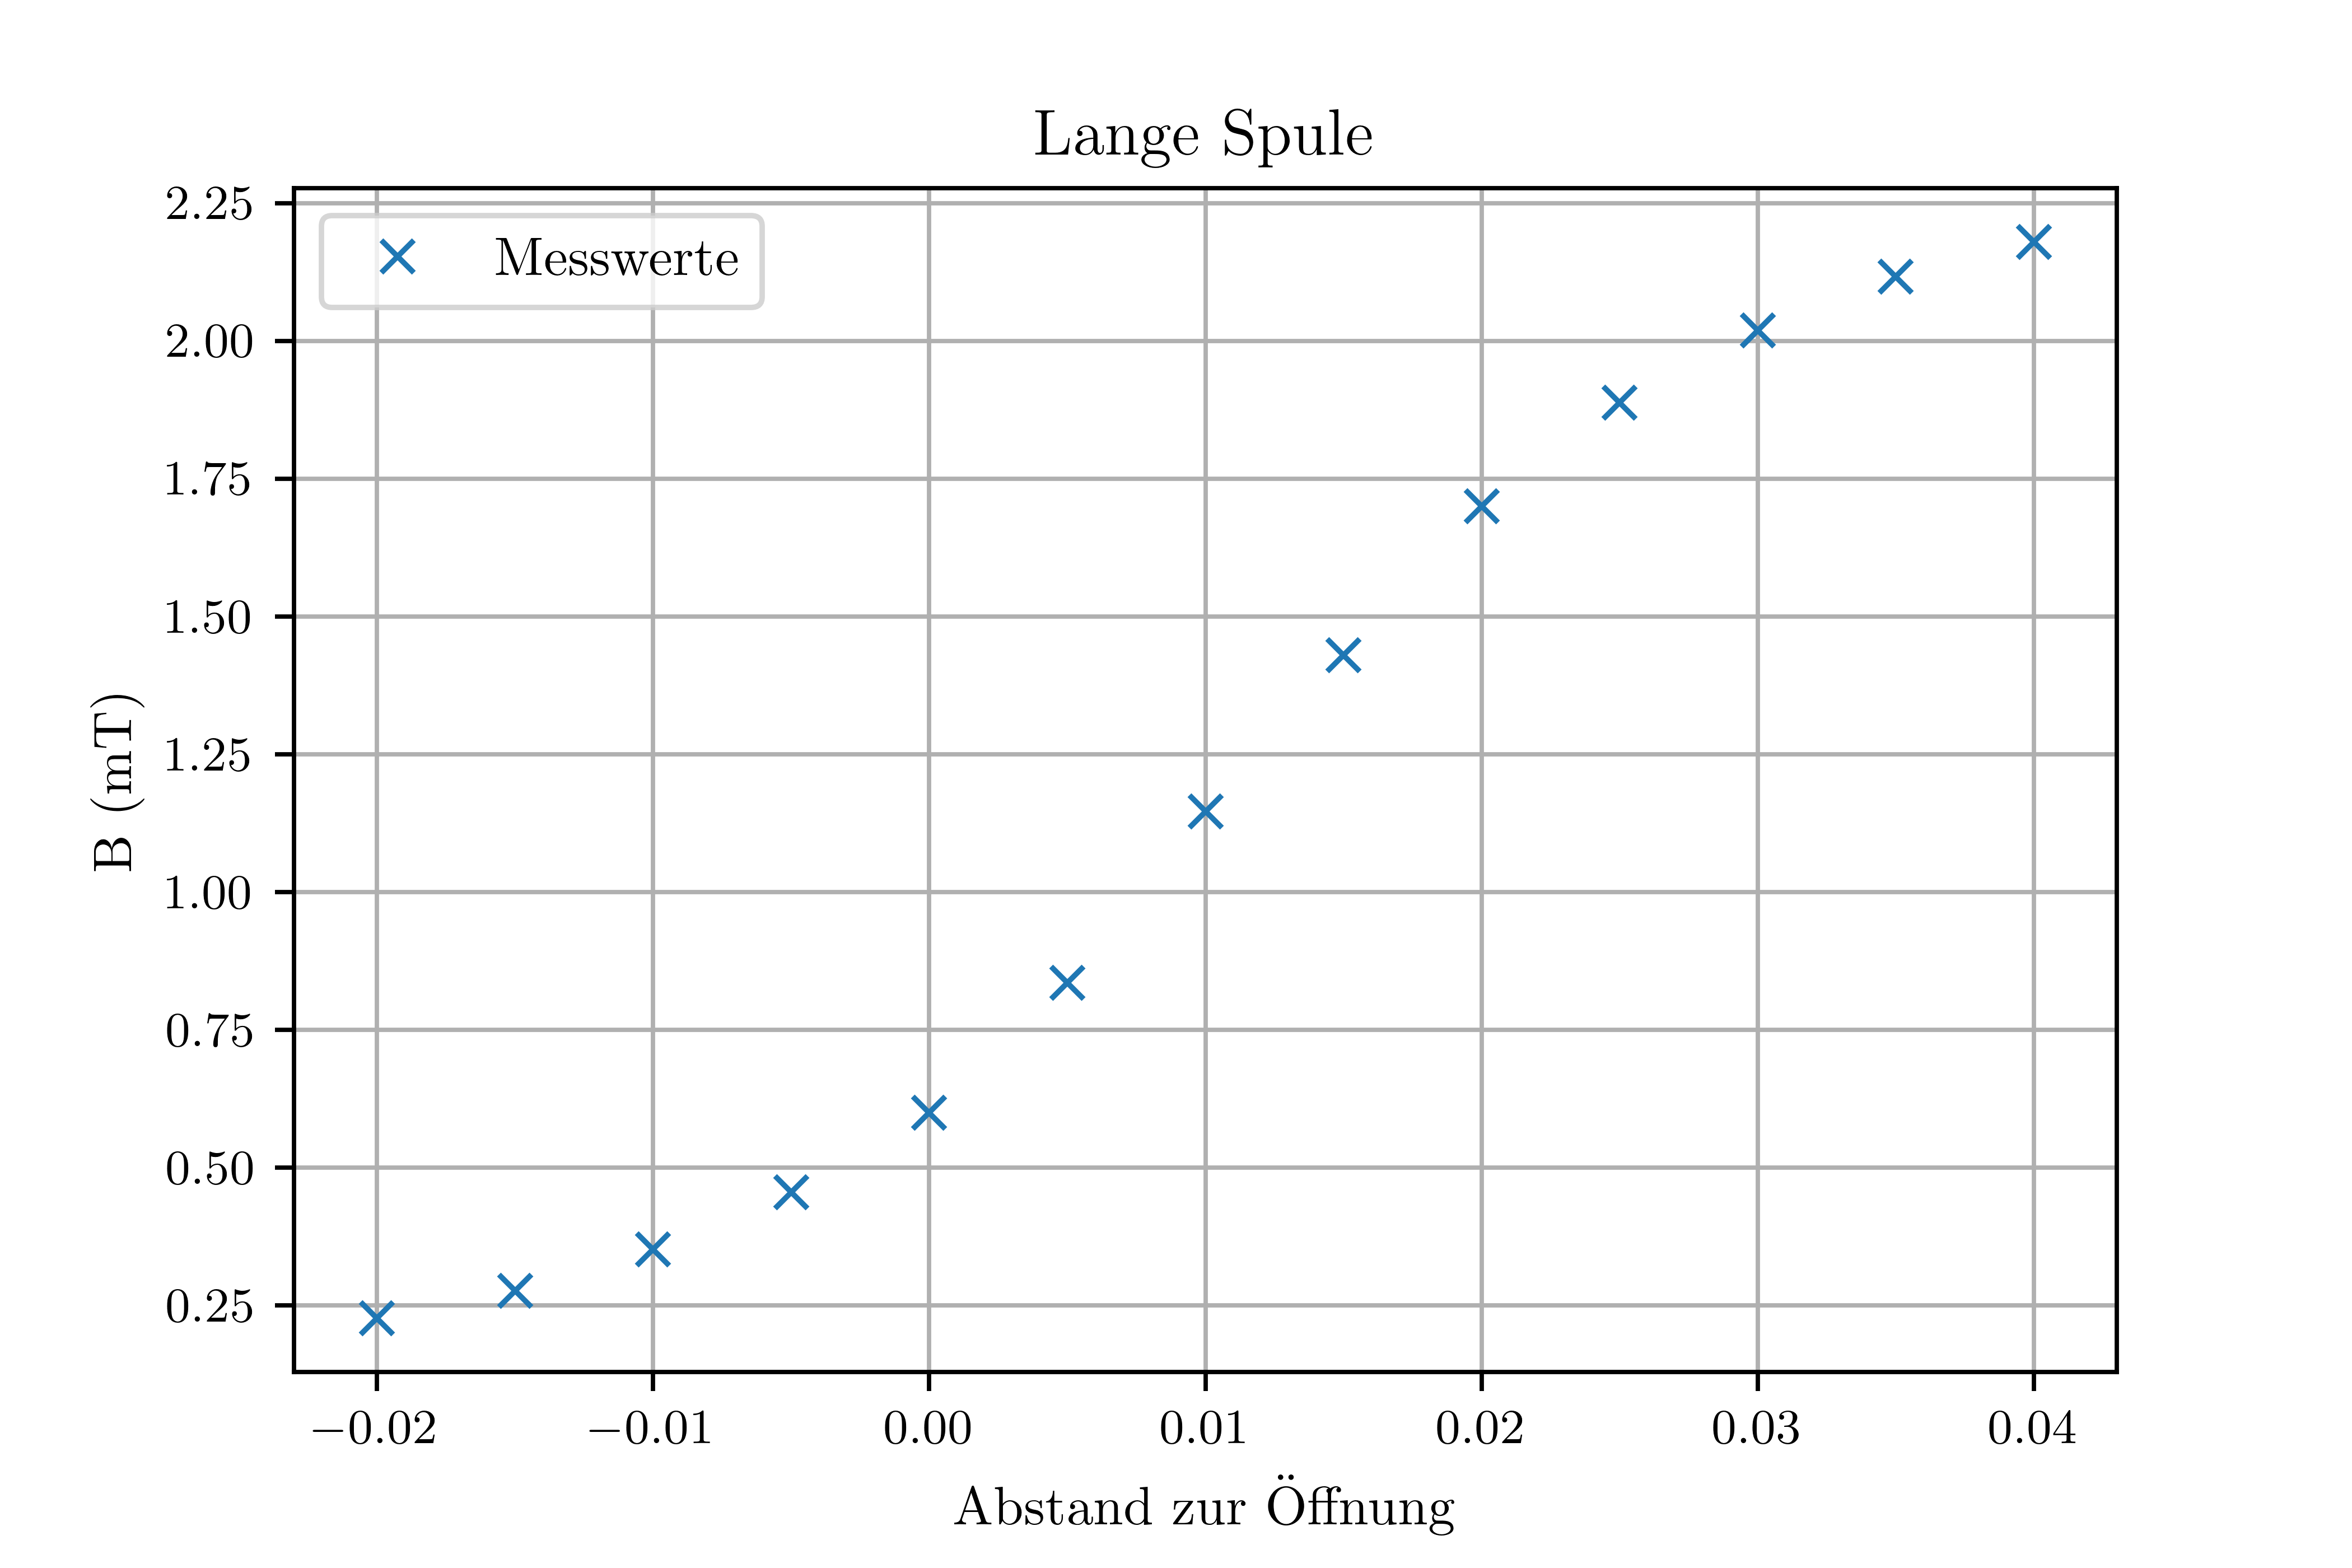
\includegraphics[width=\textwidth]{pictures/LangeSpule1.png}    %Hier fehlt noch die Beschriftung
%\end{minipage}

Es ist eine abflachende Steigung des Magnetfeldes zu erkennen. Der Theoriewert, der sich aus der Formel (\ref{eq:LangeSpule}) ergibt, lautet:
\begin{equation}
  B_{\text{LS}} = 2.31 T
\end{equation}


\subsection{Helmholtzspulenpaar}

Im folgenden sind die Messdaten für die Abstände $d_{1} = 0.012m$, $d_{1} = 0.014m$ und $d_{1} = 0.016m$ in Tabellen und Plots dargestellt.

\begin{table}
\centering
\caption{Messdaten Helmholtzspulenpaar $d_{1} = 0.012m$}
\begin{tabular}{c c}
  \toprule
   x (m) &  B (10e-3 T) \\
  \midrule
  -0.030 &        1.895 \\
  -0.025 &        1.826 \\
  -0.020 &        1.764 \\
  -0.015 &        1.705 \\
  -0.010 &        1.657 \\
  -0.005 &        1.645 \\
   0.000 &        1.632 \\
   0.005 &        1.638 \\
   0.010 &        1.660 \\
   0.015 &        1.700 \\
   0.020 &        1.754 \\
   0.025 &        1.818 \\
   0.030 &        1.890 \\
   0.090 &        1.634 \\
   0.100 &        1.390 \\
   0.110 &        1.137 \\
   0.120 &        0.915 \\
  \bottomrule
\end{tabular}
\end{table}

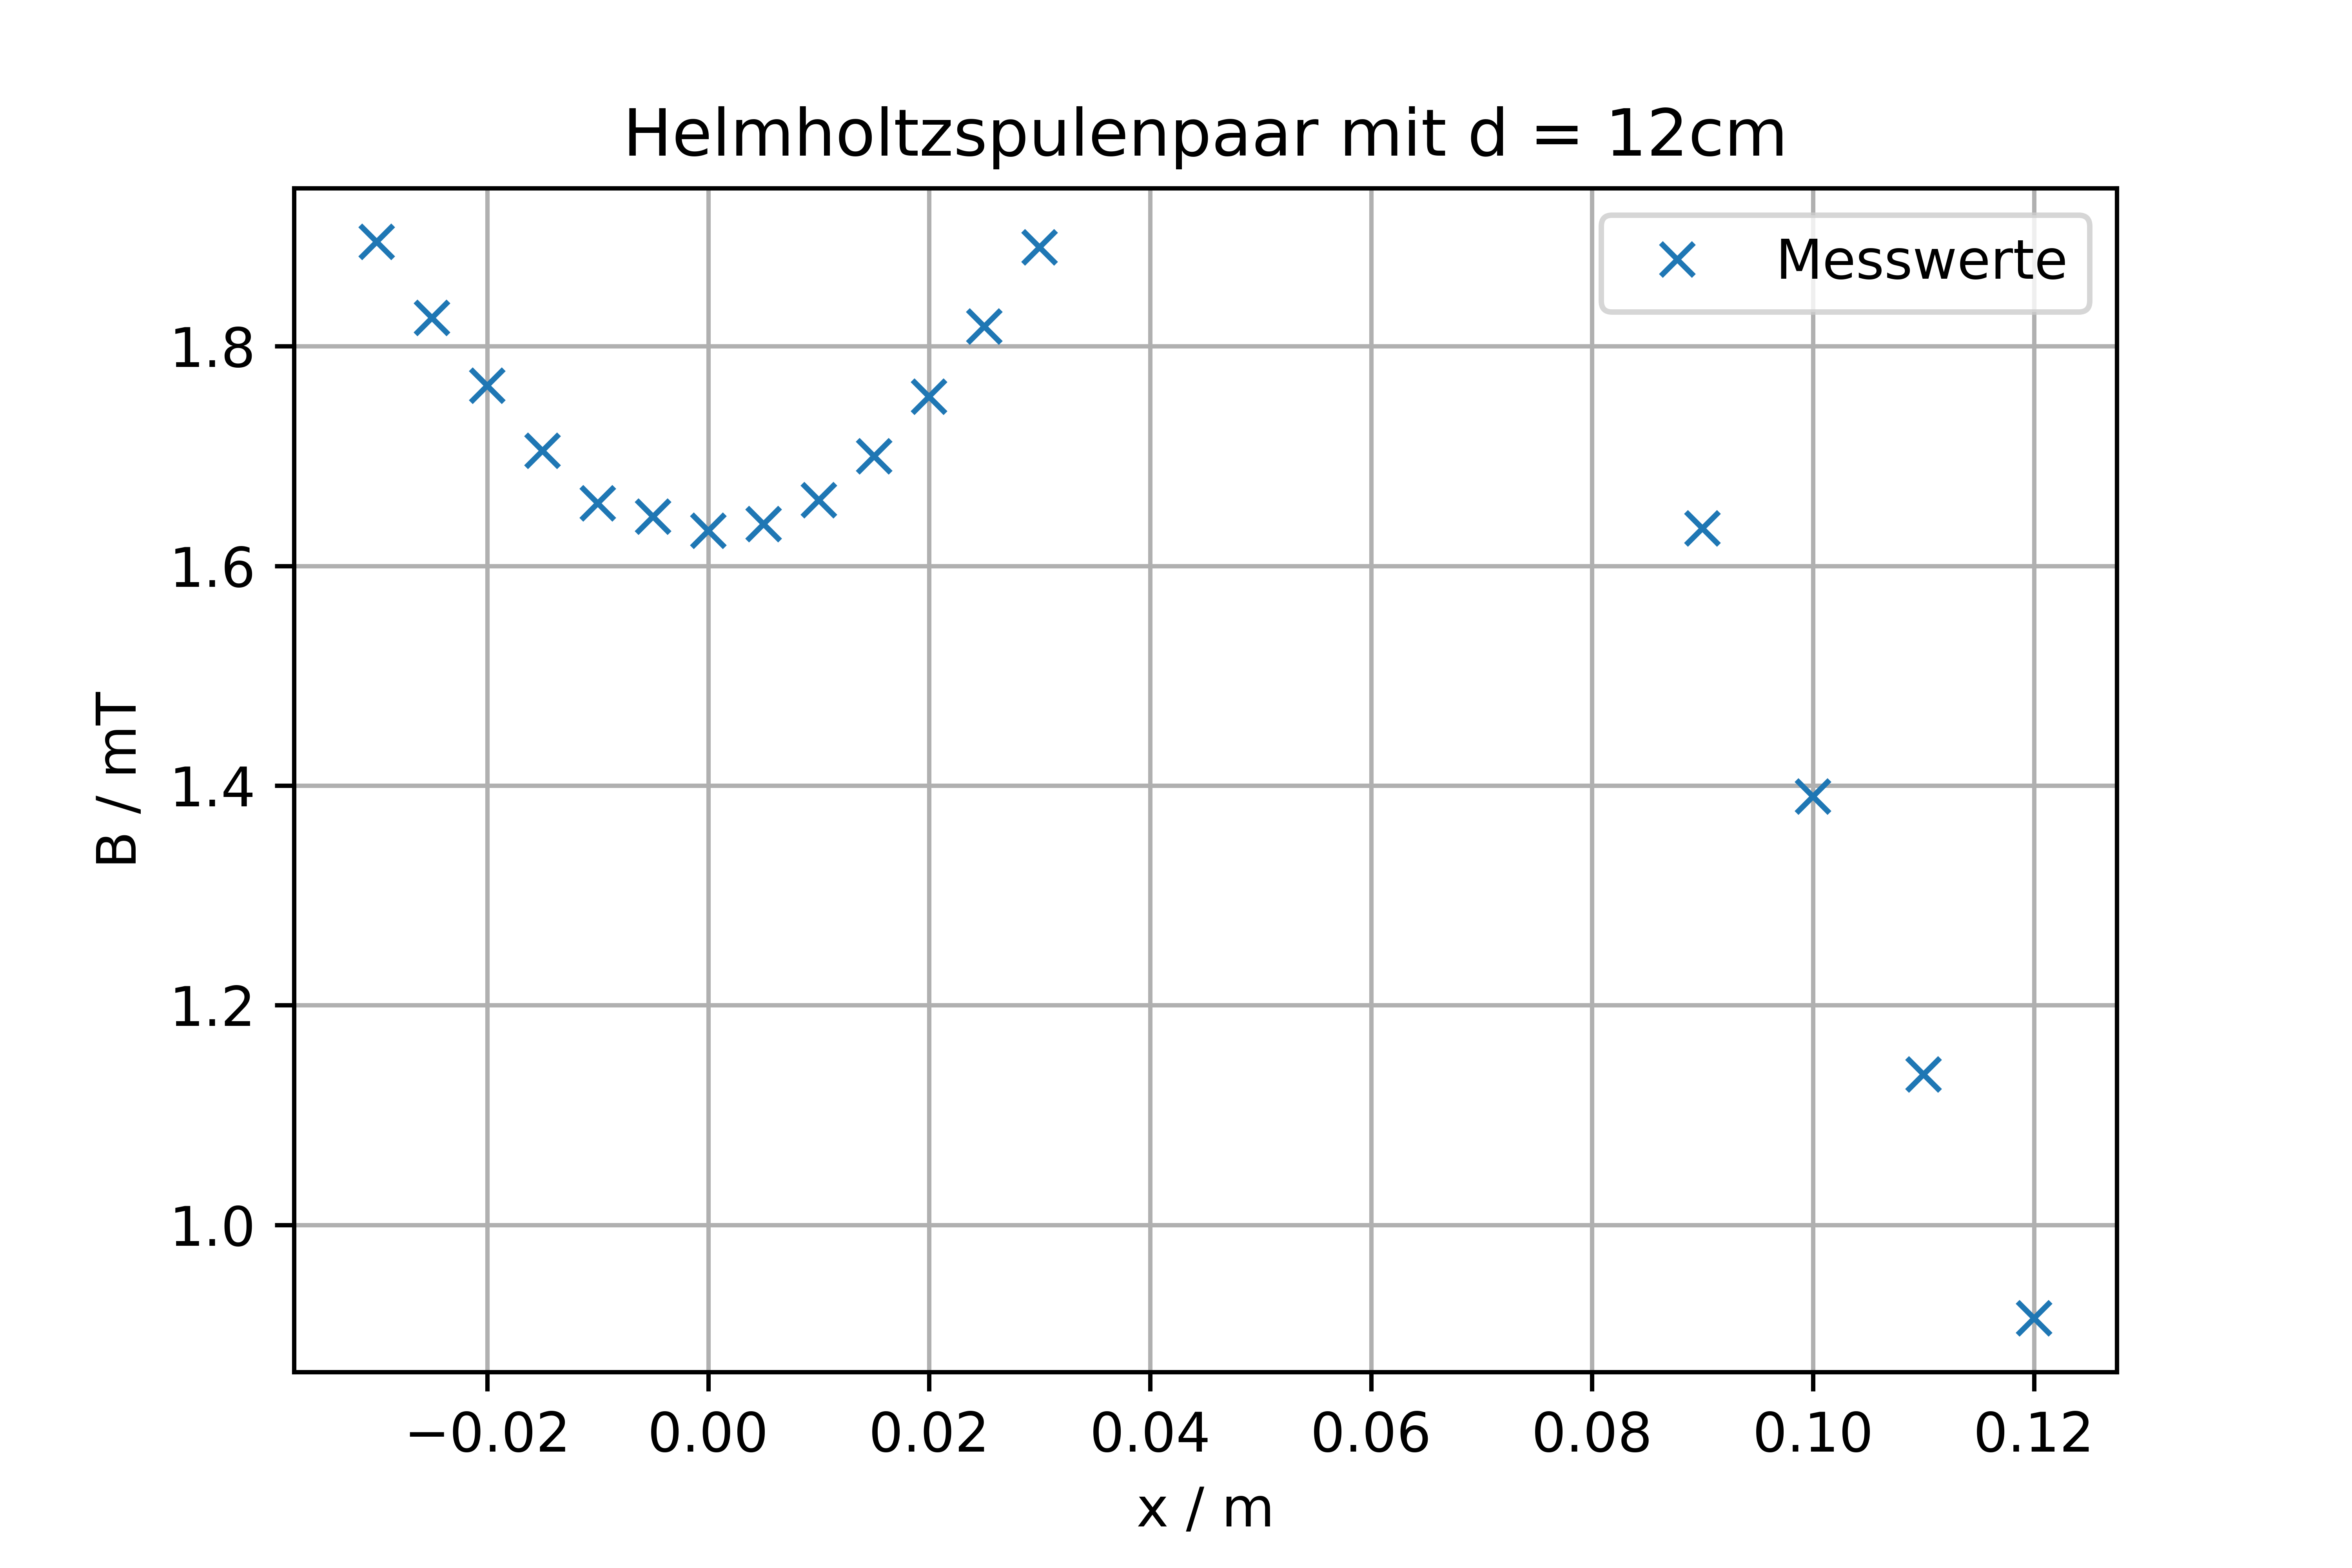
\includegraphics[width=\textwidth]{pictures/Helmholtz1.png}    %Hier fehlt noch die Beschriftung

\begin{table}
\centering
\caption{Messdaten Helmholtzspulenpaar $d_{2} = 0.014m$}
\begin{tabular}{c c}
  \toprule
   x (m) &  B (10e-3 T) \\
  \midrule
  -0.030 &        1.608 \\
  -0.025 &        1.520 \\
  -0.020 &        1.448 \\
  -0.015 &        1.394 \\
  -0.010 &        1.346 \\
  -0.005 &        1.322 \\
   0.000 &        1.312 \\
   0.005 &        1.316 \\
   0.010 &        1.314 \\
   0.015 &        1.375 \\
   0.020 &        1.437 \\
   0.025 &        1.505 \\
   0.030 &        1.572 \\
   0.100 &        1.596 \\
   0.110 &        1.332 \\
   0.120 &        1.091 \\
   0.130 &        0.875 \\
  \bottomrule
  \end{tabular}
\end{table}

\includegraphics[width=\textwidth]{pictures/Helmholtz2.png}    %Hier fehlt noch die Beschriftung


\begin{table}
  \centering
  \caption{Messdaten Helmholtzspulenpaar $d_{3} = 0.016m$}
  \begin{tabular}{c c}
    \toprule
     x (m) &  B (10e-3 T) \\
    \midrule
    -0.030 &        1.300 \\
    -0.025 &        1.225 \\
    -0.020 &        1.160 \\
    -0.015 &        1.112 \\
    -0.010 &        1.074 \\
    -0.005 &        1.054 \\
     0.000 &        1.044 \\
     0.005 &        1.049 \\
     0.010 &        1.073 \\
     0.015 &        1.106 \\
     0.020 &        1.156 \\
     0.025 &        1.210 \\
     0.030 &        1.300 \\
     0.110 &        1.546 \\
     0.120 &        1.295 \\
     0.130 &        1.060 \\
     0.140 &        0.852 \\
    \bottomrule
  \end{tabular}
\end{table}

  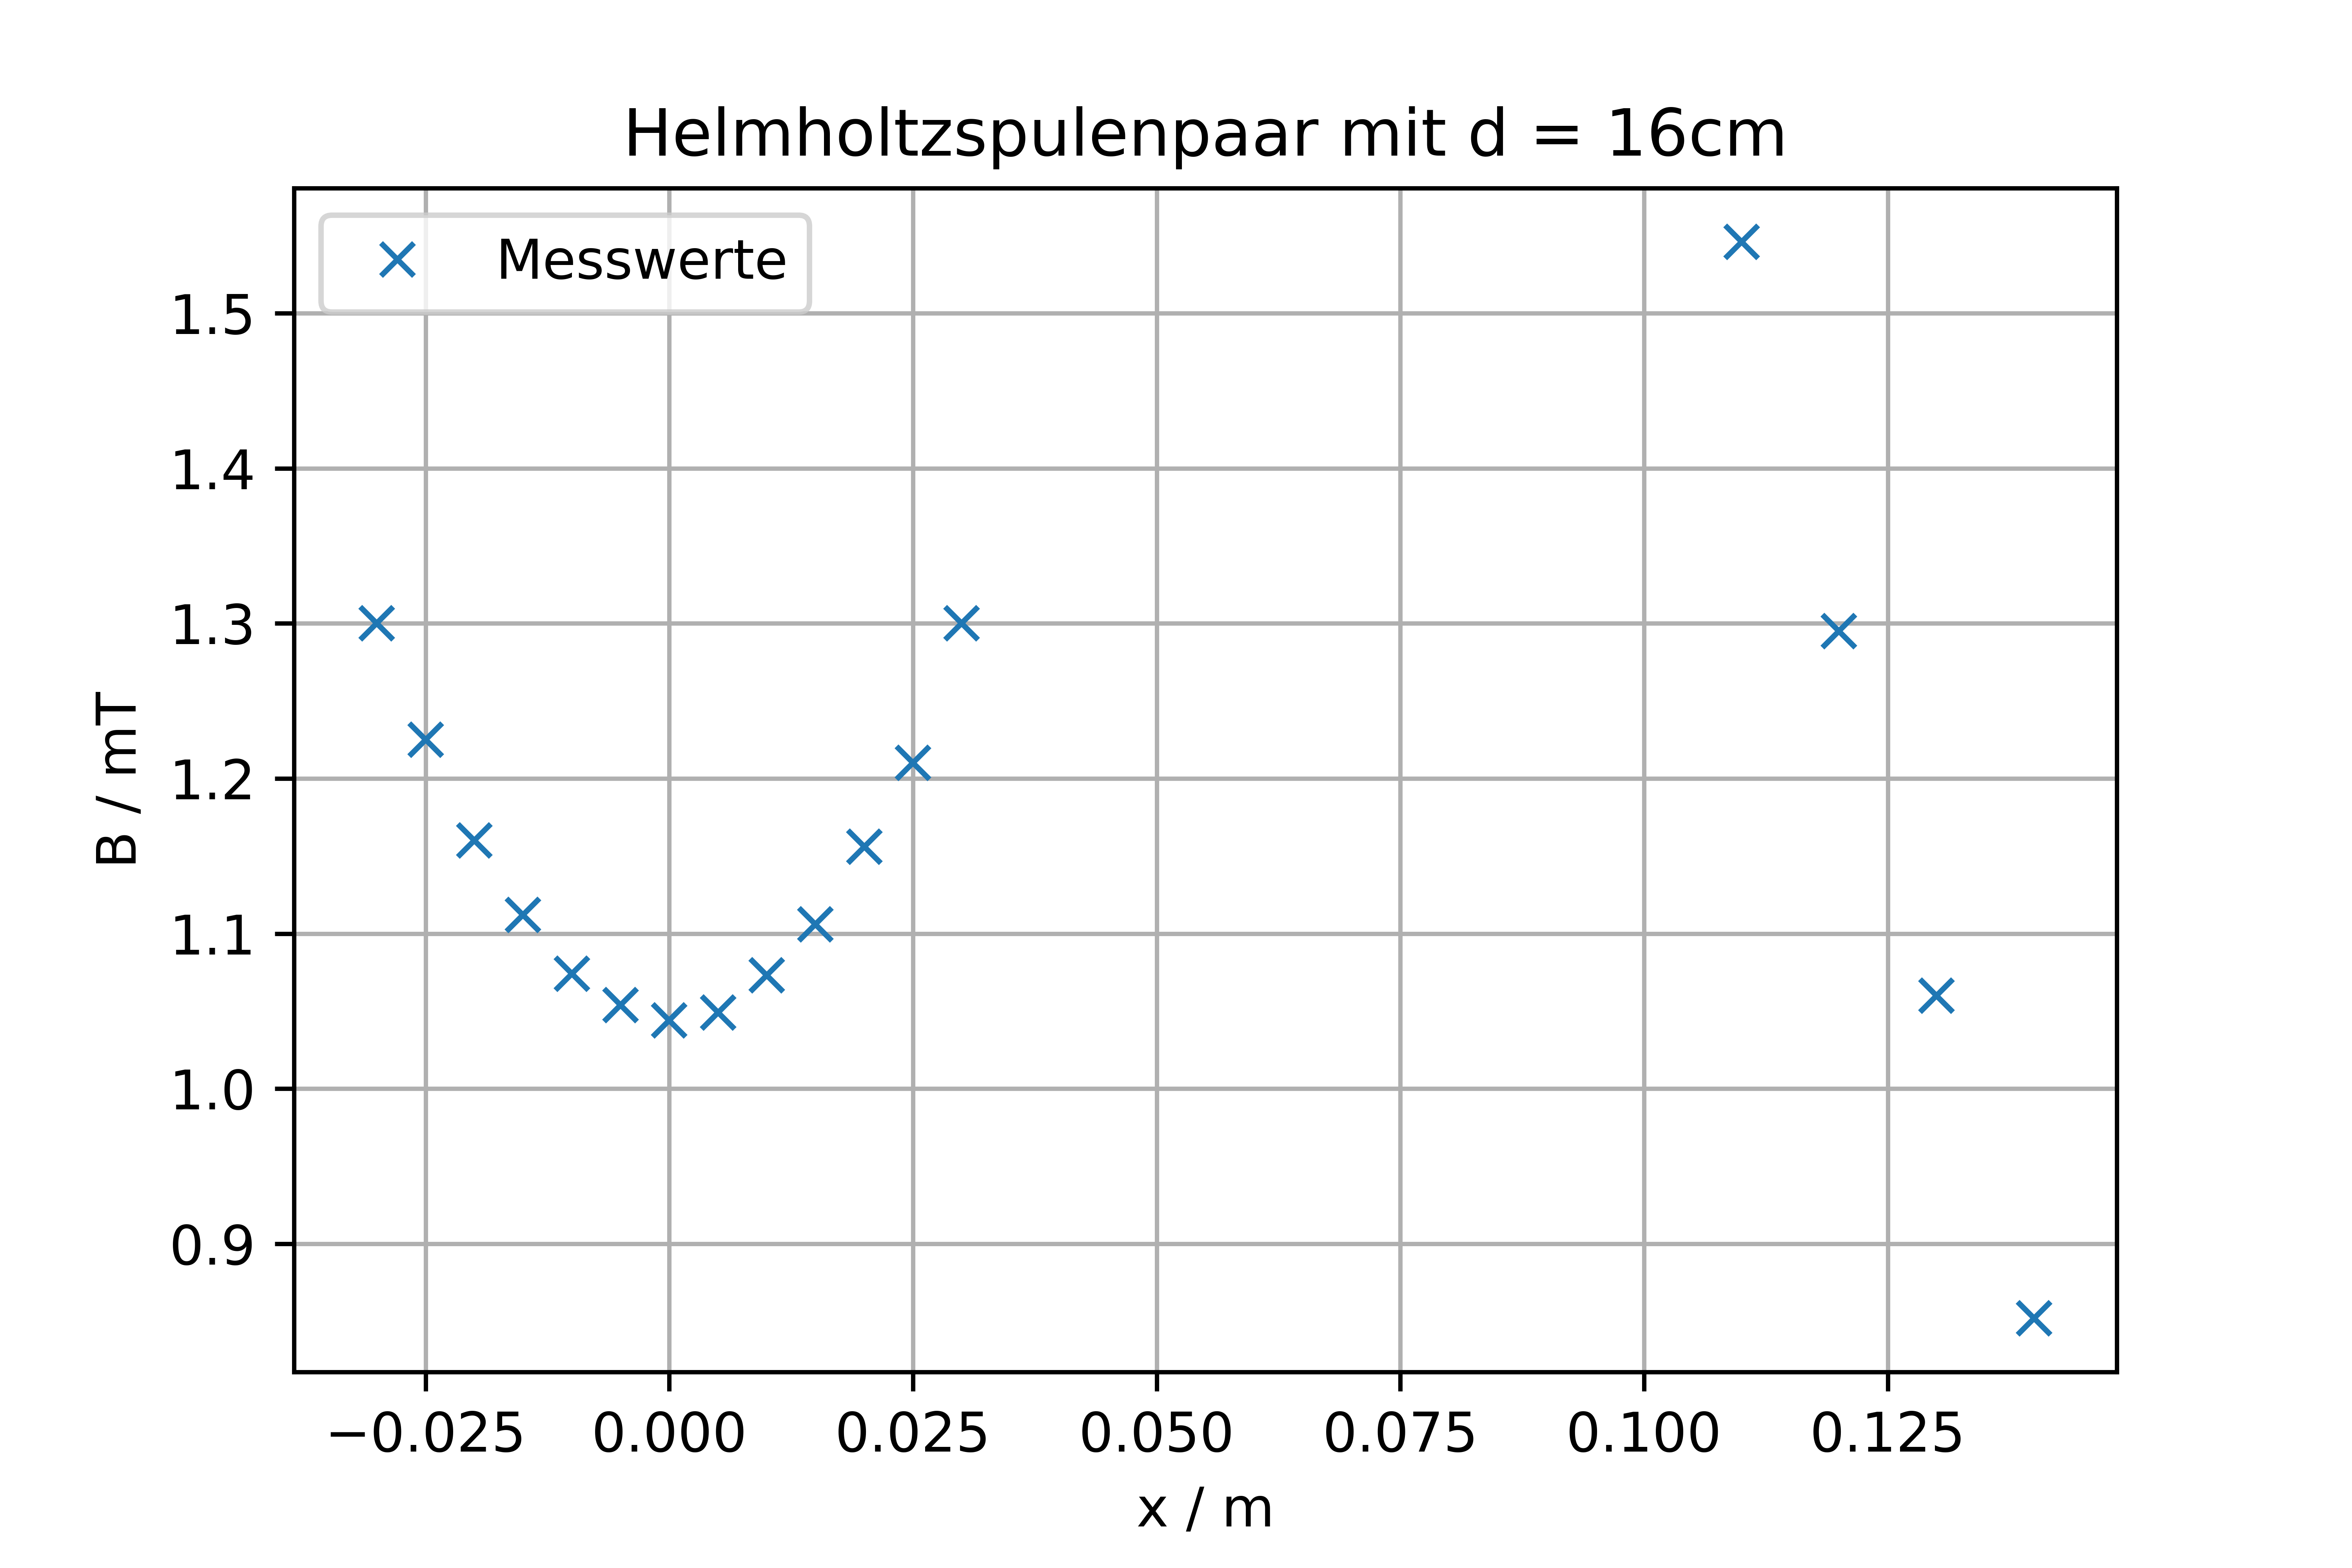
\includegraphics[width=\textwidth]{pictures/Helmholtz3.png}    %Hier fehlt noch die Beschriftung

  Aus Gleichung (\ref{eq:Helmholtzgleichung}) ergeben sich die theoretischen Vergleichswerte.
  In der Tabelle wird das Magnetfeld im Zentrum also mit der Theorie verglichen.

  \begin{table}
    \centering
    \caption{Vergleich der Messwerte mit der Theorie}
    \begin{tabular}{c c c c }
      \toprule
      $d_{i}$ & $B_{\text{errech}}$(0) (10e-3T) &  $B_{\text{gemessen}}$(0) (10e-3T) & Prozentuale Abw. (\%)\\
      \midrule
      i = 1  & 1.585 &         1.632  &     2.97 \\ 
      i = 2  & 1.247 &         1.312  &     5.21 \\ 
      i = 3  & 0.985 &         1.044  &     5.99 \\ 
      \bottomrule
    \end{tabular}
  \end{table}

\subsection{Ringspule}

Im folgenden wollen wir die Hysteresekurve der Ringspule graphisch darstellen.

\begin{table}
\centering
\caption{Messwerte der Hysterese}
\begin{tabular}{c c c c c c}
  \toprule
   I (A) &  B (10e-3 T) &  I (A) &  B (10e-3 T) &  I (A) &  B (10e-3 T)\\
  \midrule
     0 &        0.000 &         0 &      -86.000 &   0 &     -134.300 \\
     1 &       64.900 &        -1 &     -118.000 &   1 &       75.500 \\
     2 &      230.700 &        -2 &     -307.800 &   2 &      258.700 \\
     3 &      351.500 &        -3 &     -434.800 &   3 &      388.600 \\
     4 &      435.200 &        -4 &     -525.400 &   4 &      480.800 \\
     5 &      496.800 &        -5 &     -579.900 &   5 &      543.100 \\
     6 &      542.900 &        -6 &     -588.300 &   6 &      586.900 \\
     7 &      582.100 &        -7 &     -625.000 &   7 &      626.700 \\
     8 &      613.800 &        -8 &     -657.200 &   8 &      659.000 \\
     9 &      641.500 &        -9 &     -684.900 &   9 &      686.400 \\
    10 &      666.600 &       -10 &     -714.100 &  10 &      711.800 \\
     9 &      653.300 &        -9 &     -696.900 &  -  &        -     \\
     8 &      638.700 &        -8 &     -679.200 &  -  &        -     \\
     7 &      617.800 &        -7 &     -661.400 &  -  &        -     \\
     6 &      596.000 &        -6 &     -637.900 &  -  &        -     \\
     5 &      565.700 &        -5 &     -610.000 &  -  &        -     \\
     4 &      529.600 &        -4 &     -576.000 &  -  &        -     \\
     3 &      484.400 &        -3 &     -535.200 &  -  &        -     \\
     2 &      420.700 &        -2 &     -471.400 &  -  &        -     \\
     1 &      300.000 &        -1 &     -345.300 &  -  &        -     \\
  \bottomrule
  \end{tabular}
\end{table}

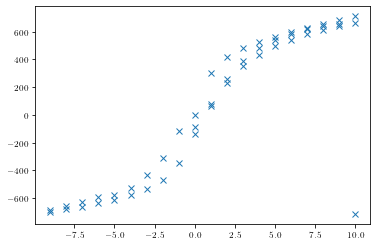
\includegraphics[width=\textwidth]{pictures/HysteresekurveGemessen3.png}    %Hier fehlt noch die Beschriftung

Aus den Messwerten lassen sich Remanenz und Koerzitivkraft angeben.
Dabei wird die Koerzitivkraft aus der Abbildung abgelesen.
\begin{align*}
  B_{r,1} &= -86 mT &  B_{r,2} &= 134.3 mT \\
  H_{c,1} &\approx 0.5A & H_{c,2} &\approx 0.7A
\end{align*}